
\chapter{Getting started}

\section{Installation}

Before installing \xlp you need to install python. \xlp has been tested with version 2.5 of python. We suggest you to install this version.

\

Once python is installed, go to the directory {\it I:/Bjb\_App/Arena/Quants/xlpython}. Open excel, menu Tools -> Addins, install xlpython.xll (say yes to copy on your computer). 

\

Open the file xlp-example.xll to check the installation. 

\section{\xlp Concept}


\xlp is an Excel add-in. Which provides some new functions available into the function wizard. 

\xlp implements the  {\it Object Handler Concept} using the functionalitiy of Python. Is to say that you will create python object instances directly into a worksheet, instances can in turn be used for future calculations.

\

An example is always better.

\

Imagine that you have a data set which represents a rate term structure:

\begin{center}
\begin{tabular}{c|c}
\bf{Maturity (year fraction)} & rate \\
\hline\\
1.00 & 3.60\% \\
2.00 & 4.60\% \\
3.00 & 5.60\% \\
4.00 & 6.60\% 
\end{tabular}
\end{center}

Your aim is to interpolate the rate term structure linearly for a set of times ${1.5, 2.5, 3.5}$.

\

One solution will be to use a interpolation function, named {\it linear\_interpolate}, that will take 3 argument vectors: the rates, the times and the time where you want to interpolate.  

\begin{center}
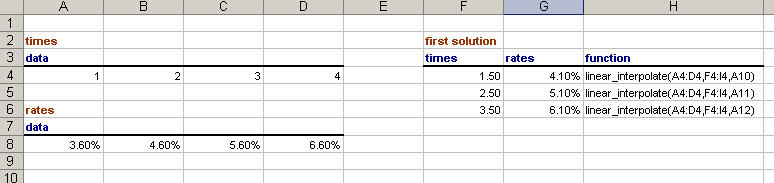
\includegraphics[width=16cm]{images/intex1.jpg}
\end{center}

This solution is simple but you can immediately see that this has a lot of drawbacks:

\begin{itemize}
\item You have to specify the input data every time you want to interpolate. That increase the possibility to make mistakes.
\item For each interpolation, you need to perform the same calculation on the same data even if they do not change, that cause a performance decrease. 
\end{itemize}

\

Another solution is to use objects and keep a record of theses objects into Excel.

\begin{center}
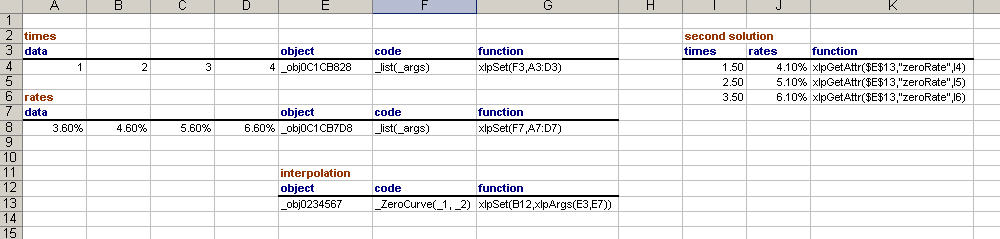
\includegraphics[width=16cm]{images/intex2.jpg}
\end{center}

As seen on the figure above, first we create objects which represents times and rates. With this two objects we compose a {\it ZeroCurve} object. Then we use this object to obtain the value of the interpolation.

This solution is more complex than the first use but it is more efficient.

